\setchapterpreamble[u]{\margintoc}
\chapter{基础题目}
\labch{Basic}
\section{基础知识}
符号:
\begin{description}
	\item[$f^n(x)$] 表示$f$的$n$次复合,$\underbrace{f(f(\cdots f(x)))}_{n\text{层}}$。特别地,$f^0(x)=x$。 
	\item[$\binom{m}{n}$] 表示$m$中取$n$的组合数,$\binom{m}{n}=C_m^n=\dfrac{m!}{n!(m-n)!}$ 。
\end{description}
常见函数的导数:\\
\begin{center}
	\begin{tabular}{lll}
		\hline
		函数&导函数&定义域\\
		\hline
		$ax^n$&$anx^{n-1}$&$x\in\mathbb{R},n\neq 0$\\
		$a^x$&$a^x\ln a$&$x \in \mathbb{R},a\neq 0$\\
		$e^x$&$e^x$&$x \in \mathbb{R}$\\
		$\ln x$&$\dfrac{1}{x}$&$x \in (0,+\infty)$\\
		$\log_a{x}$&$\dfrac{1}{x\ln a}$&$x,a \in (0,+\infty)$\\
		$\sin x$&$\cos x$&$x\in \mathbb{R}$\\
		$\cos x$&$-\sin x$&$x\in \mathbb{R}$\\
		$\tan x$&$\dfrac{1}{\cos^2 x}$&$x \neq \dfrac{(2n+1)\pi}{2}, n \in \mathbb{Z}$\\[0.5em]
		\hline
	\end{tabular} 
\end{center}
复合函数的导数:\par\vspace{1em}
\begin{tabular}{ccccc}
	\hline\\[-1em]
	函数&$f(g(x))$&$f(x)+g(x)$&$f(x)g(x)$&$\dfrac{f(x)}{g(x)}$\\[1em]
	\hline\\[-1em]
	导函数&$g'(x)f'(g(x))$&$f'(x)+g'(x)$&$f'(x)g(x)+f(x)g'(x)$&$\dfrac{f'(x)g(x)-f(x)g'(x)}{[g(x)]^2}$\\[1em]
	\hline
\end{tabular}\par\vspace{1em}
函数积的多次导数(莱布尼兹公式):
$$\left[f(x)g(x)\right]^{(n)}=\sum_{k=0}^n \binom{n}{k} f^{(k)}(x)g^{(n-k)}(x)=C_n^0f(x)g^{(n)}(x)+C_n^1f'(x)g^{(n-1)}(x)+\cdots+C_n^nf^{(n)}(x)g(x)$$
\section{函数的概念}

\begin{que}
	已知函数$f(x)$定义域为$\left[-\dfrac{1}{2},\dfrac{3}{2}\right]$,$a>0$,求函数$g(x)=f(ax)+f\left(\dfrac{x}{a}\right)$的定义域。
\end{que}
\sol 过程略。\begin{enumerate}
	\item 当$a\geqslant 1$时,所求定义域$\res{\left[-\dfrac{1}{2a},\dfrac{3}{2a}\right]}$;
	\item 当$0<a<1$时,所求定义域$\res{\left[-\dfrac{a}{2},\dfrac{3a}{2}\right]}$。\hfill\tg{定义域}\easy
\end{enumerate} 

\begin{que}
	求下面函数的值域:(1)$y=\dfrac{2\sin x-1}{2\sin x+1}$\ (2)$y=\dfrac{e^x-e^{-x}}{e^x+e^{-x}}$\ \\[0.5em](3)$y=(x+1)(x+2)(x+3)(x+4),x\in[-3,3]$
\end{que}
\sol \begin{enumerate}
	\item \blue{(方法一)}\sidenote{但凡有单值反函数,那末反函数的定义域即为函数的值域,反函数的值域即为函数的定义域。}反解$\sin x$得$\sin x= \dfrac{1+y}{2(1-y)}$,由$\sin x\in[-1,1]$知,严格地,$$|\sin x|=\left|\dfrac{1+y}{2(1-y)}\right|\leqslant 1\ \Leftrightarrow\ (1+y)^2\leqslant 4(1-y)^2\ \Leftrightarrow\ \res{y\in\left(-\infty,\dfrac{1}{3}\right]\cup[3,+\infty)}$$
	\blue{(方法二)}记$t=\sin x\in[-1,1]$,则$$y=\dfrac{2t-1}{2t+1}=1-\dfrac{2}{2t+1}\res{\in\left(-\infty,\dfrac{1}{3}\right]\cup[3,+\infty)}$$
	\item 两种方法同上,此处不赘述。$\res{y\in(-1,1)}$。
	\item 对称展开得$y=(x^2+5x+4)(x^2+5x+6)=(t+4)(t+6)=(t+5)^2-1$,其中$t=x^2+5x\in\left[-\dfrac{25}{4},24\right]$,结合二次函数图像可知$y=(t+5)^2-1\in\res{[-1,840]}$。\par\hfill\tg{反函数\ 值域}\easy
\end{enumerate}

\begin{que}
	求下列函数的值域:(1)$f(x)=-\dfrac{x^2-x+2}{x^2+2}$\ (2)$f(x)=x-\sqrt{1-x^2}$
\end{que}
\sol \begin{enumerate}
	\item \blue{(方法一)}$f(x)=-\dfrac{x^2-x+2}{x^2+2}=\dfrac{1}{\dfrac{2}{x}+x}-1$,分母是对勾函数\sidenote{当我们上下同除$x$时,事实上假定了$x\neq 0$,因此计算后须对$x=0$时的取值进行补充。这样做是无妨的,原因有二,一是$f(x)$是连续的,二是我们完全可以补充$\dfrac{1}{\infty}=0$。},其值域为$\dfrac{2}{x}+x\in(-\infty,-2\sqrt{2})\cup(2\sqrt{2},+\infty)$,另外$f(-1)=0$,因此得值域$\res{\left[-1-\dfrac{\sqrt{2}}{4},-1+\dfrac{\sqrt{2}}{4}\right]}$。\par
	\blue{(方法二)}	注意到分母不为$0$。记$f(x)=y$,则原式$\ \Leftrightarrow\ (y+1)x^2-x+(2y+2)=0$,视之为关于$x\in\mathbb{R}$的二次函数\sidenote{形如$f(x)=\dfrac{a_1x^2+b_1x+c_1}{a_2x^2+b_2x+c_2}$和$f(x)=ax+b+c\sqrt{dx^2+ex+f}$的函数式均可尝试用判别式的方法求值域。},那末$$\Delta=1-4(y+1)(2y+2)\geqslant 0\ \Leftrightarrow\ y\in\res{\left[-1-\dfrac{\sqrt{2}}{4},-1+\dfrac{\sqrt{2}}{4}\right]}$$
	\begin{marginfigure}
		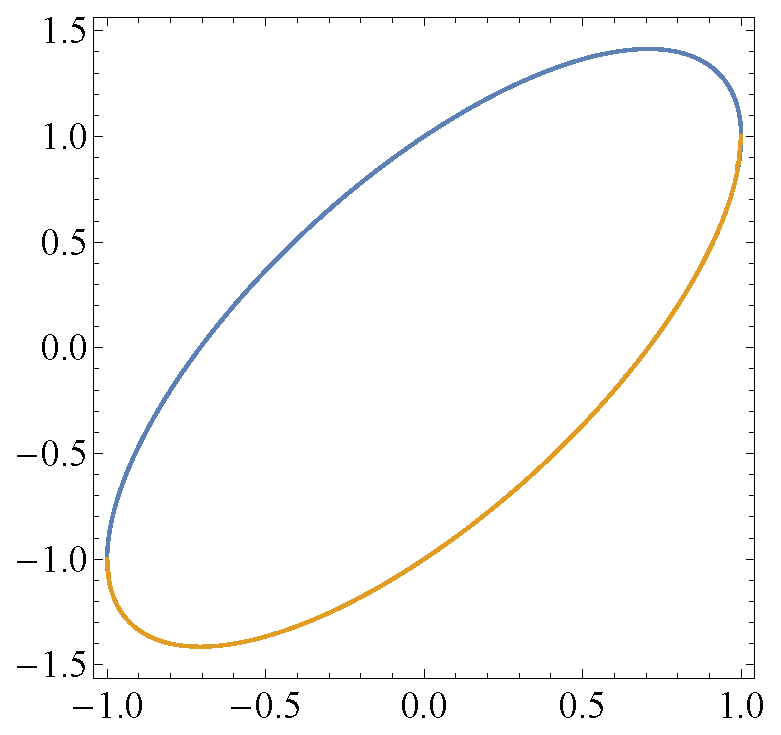
\includegraphics{Figure-3.eps}
		\caption{$2x^2-2x y+y^2=1$的图像。橙色部分即为(2)中$f(x)$的图像。}
	\end{marginfigure}
	\item \blue{(方法一)}设$x=\sin t\in[-1,1]$\sidenote{为何设三角函数对于类似形式的函数可以起到等价化简的作用?因为这原本就是二次圆锥曲线的变形,本题(2)中的函数即是旋转的椭圆。},则$f(x)=\sin t-|\cos t|\in\res{[-\sqrt{2},1]}$。\par
	\blue{(方法二)}易知$f(x)$在$[0,1]$上有$f(x)\geqslant f(-x)$且单调增,$x\in[-1,1]$,因此严格地$f(x)\leqslant f(1)=1$。又$$(y-x)^2=1-x^2\ \Leftrightarrow\ 2x^2-2xy+y^2-1=0\ \\\Rightarrow\ \Delta=8-4y^2\geqslant 0\ \Leftrightarrow\ f(x)=y\in[-\sqrt{2},\sqrt{2}]$$
	注意到$f\left(-\dfrac{\sqrt{2}}{2}\right)=-\sqrt{2}$,$f(x)$连续\sidenote{求最值和求值域是不同的,函数不一定能取到最大值和最小值之间的值,然而函数必然可以取到值域中的所有值。},故值域$\res{f(x)\in[-\sqrt{2},1]}$。
\end{enumerate}\par\hfill\tg{判别式\ 值域}\easy

\begin{que}
	\begin{enumerate}
		\item 已知函数$f(x)=\log_a\left(x+\dfrac{a}{x}-4\right)$的定义域为$\mathbb{R}$,其中$a>0$,$a\neq 1$,求实数$a$的取值范围。
		\item 已知函数$f(x)=\log_3\dfrac{mx^2+8x+n}{x^2+1}$的定义域为$\mathbb{R}$,值域为$[0,2]$,求$m,n$的值。
		\item 设函数$f(x)=\log_3\dfrac{bx^2+ax+b}{x^2+x+1}$,已知$a>b$,函数的值域为$(-\infty,0]$,求$a$的取值范围。
	\end{enumerate}
\end{que}
\sol \begin{enumerate}
	\item 值域为$\mathbb{R}$意味着$x+\dfrac{a}{x}-4$值域包含$\mathbb{R}^+$,又$a>0$,故这是一个对勾函数,其最小值为$x+\dfrac{a}{x}-4\geqslant 2\sqrt{x\cdot\dfrac{a}{x}}-4=2\sqrt{a}-4$,那末只需使$2\sqrt{a}-4\leqslant 0\Rightarrow\res{a\in(0,1)\cup(1,4]}$。
	\item 由于$f(x)$定义域为$\mathbb{R}$,故$\forall x\in \mathbb{R}$,恒有$$\dfrac{mx^2+8x+n}{\underbrace{x^2+1}_{>0}}>0\ \Leftrightarrow\ \text{\footnotesize 分母}\Delta=64-4mn<0,m>0$$
	又根据值域有\sidenote{此过程中暗含使用了$x\in\mathbb{R}$这一条件,因此我们可以毫无顾虑的使用判别式计算。同时闭区间端点对应的是边界条件,放在不等式上意味着「取等」。}$$\begin{aligned}\dfrac{mx^2+8x+n}{x^2+1}=k\in[1,9]\ &\Leftrightarrow\ k^2-(m+n)k+mn-16\leqslant 0,\forall k\in[1,9]\ \\
		&\Rightarrow\ m+n=10,mn-16=9\ \Rightarrow\ \res{m=n=5}\end{aligned}$$
	\item 由题条件\sidenote{本小题对定义域没有说明和限制,但并不意味着定义域为$\mathbb{R}$。},$$\dfrac{bx^2+ax+b}{\underbrace{x^2+x+1}_{>0}}=k\in(0,1]\ \Rightarrow\ (b-k)x^2+(a-k)x+(b-k)=0$$当$k\in(0,1]$时恒有解,$k>1$时无解。因此
	$$\begin{aligned}&\quad\ \forall k\in(0,1],\ \Delta=(a-k)^2-4(b-k)^2\geqslant 0,\text{且}k=1\text{处取等,下同}\\
	&\Leftrightarrow\ \forall k\in(0,1],\ \left(k-\dfrac{a+2b}{3}\right)(k-(2b-a))\geqslant 0\end{aligned}$$
	由于$a>b$,故$\dfrac{a+2b}{3}>2b-a$,$$\left\{\begin{aligned}&\dfrac{a+2b}{3}=1\\& 2b-a\leqslant 0\end{aligned}\right.\ \Rightarrow\ \res{a\geqslant\dfrac{3}{2}}$$
\end{enumerate}\par\hfill\tg{复合函数}\normal

\begin{que}
	已知$f(x)=\sqrt{4-x^2}$在闭区间$M$上的反函数是其本身,求$M$的取值集合。
\end{que}
\sol 显然$f(x)$函数图像为半径为$2$,圆心在原点的圆的上半部分。结合函数与其反函数图像的几何关系\sidenote{函数与其反函数关于直线$x=y$镜像对称。},可知$M$的取值集合为$\res{M\in\left\{[2\sin\theta,2\cos\theta]:\theta\in\left[0,\dfrac{\pi}{4}\right]\right\}}$。\par\hfill\tg{反函数\ 圆}\easy

\begin{que}
	设定义域为$\mathbb{R}$的函数$f(x),g(x)$均有反函数,且函数$f(x-1)$和$g^{-1}(x-2)$的图像关于直线$y=x$对称,若$g(5)=2021$,求$f(4)$的值。
\end{que}
\sol 由题意$(5,f(4))$与$(f(4),g^{-1}(f(4)-2))$关于$y=x$对称,故$g^{-1}(f(4)-2)=5$,由于$g(x)$有反函数,故$g$为双射\sidenote{\textbf{双射:}若关于映射$f:A\rightarrow B$有以下两特点,则称映射$f$为双射,也即「一一映射」:
\begin{enumerate}
	\item $\forall y\in B,\exists x\in A,\text{\ s.t.\ }f(x)=y$(满射)
	\item 若$x_1\in A,x_2\in A,f(x_1)=f(x_2)$,则必有$x_1=x_2$(单设)
\end{enumerate}若一个函数有反函数,即一个映射有它的逆,那末它必是双射。},因此$f(4)-2=2021\Rightarrow\res{f(4)=2023}$。\par\hfill\tg{反函数}\easy

\begin{que}
	设函数$f:\mathbb{R}\rightarrow\mathbb{R}$满足$f(0)=1$,且$\forall x,y\in\mathbb{R}$都有$f(xy+1)=f(x)f(y)-f(y)-x+2$,求$f(x)$的表达式。
\end{que}
\sol 令$x=y=0$,可得$f(1)=2$;令$y=0$,可得$f(1)=2=f(x)f(0)-f(0)-x+2=f(x)-x+1\Rightarrow\res{f(x)=x+1}$。\par\hfill\tg{抽象函数}\easy

\begin{que}
	设定义在整数集上的函数$f$满足$f(n)=\left\{ \begin{aligned}
		&n+5&n<2000\\&f(f(n-8))&n\geqslant 2000
	\end{aligned}\right.$,求$f(4096)$。
\end{que}
\sol 我们使用符号$f^k(x)$表记$\overbrace{f(f(f(\cdots f(x))))}^{k\text{次}f\text{复合}}$,那末
$$\begin{aligned}
	&\quad\ f(4096)=f^2(4088)=\cdots=f^{263}(2000)=f^{264}(1992)\\
	&=f^{262}(2002)=f^{263}(1994)=f^{261}(2004)=f^{262}(1996)=f^{261}(2001)\\
	&=f^{262}(1993)=f^{260}(2003)=f^{261}(1995)=f^{260}(2000)\end{aligned}
	$$
	这里我们得到了第一个周期$f^{263}(2000)=f^{260}(2000)$,因此可知$\forall n\geqslant 2000,k\in\mathbb{Z}$,$f^{k+3}(n)=f^k(n)$,因此$f(4096)=f^{261}(2004)=f^0(2004)=\res{2004}$。
	事实上可以求出,$\forall n\geqslant 2000$,$f(n)=2002+(n+1)\%3$,其中「\%」为取余符号。\par\hfill\tg{抽象函数}\normal

\begin{que}
	已知函数$f(x)=\dfrac{2x^2+bx+c}{x^2+1}$的值域为$[1,3]$,其中$b<0$。
	\begin{enumerate}
		\item 求实数$b,c$的值。
		\item 判断$F(x)=\lg f(x)$在$[-1,1]$上的单调性,并给出证明。
		\item 若$t\in\mathbb{R}$,求证:$\lg\dfrac{7}{5}\leqslant F\left(\left|t-\dfrac{1}{6}\right|-\left|t+\dfrac{1}{6}\right|\right)\leqslant\lg\dfrac{13}{5}$。
	\end{enumerate}
\end{que}
\sol \begin{enumerate}
	\item 记$y=f(x)$,定义域$x\neq\pm 1$。整理得$(y-2)x^2-bx+(y-c)=0\ \Rightarrow\ \Delta=b^2-4(y-2)(y-c)\geqslant 0$,由于$y=f(x)$的值域为$[1,3]$,因此$\Delta|_{y=1}=\Delta|_{y=3}=0\ \Rightarrow\ \res{b=-2,c=2}$。
	\item 由于$\lg x$是增函数,因此其增减性与$f(x)$一致。$f'(x)=\dfrac{2(x^2-1)}{(x^2+1)^2}<0$,因此$F(x)=\lg x$在$[-1,1]$上单调减。
	\item 根据$F(x)$的递减性,只需找到$h(t)=\left|t-\dfrac{1}{6}\right|-\left|t+\dfrac{1}{6}\right|$的值域。首先$h(t)$是连续的,$$h(t)\leqslant\left|\left(t-\dfrac{1}{6}\right)-\left(t+\dfrac{1}{6}\right)\right|=\dfrac{1}{3}\qquad\footnotesize{\text{当}t=-\dfrac{1}{6}\text{时取等}}$$由于$h(t)$是奇函数,因此其最小值为$\min h(t)=-\max h(t)=-\dfrac{1}{3}$。综上,$${\lg\dfrac{7}{5}}=F\left(\dfrac{1}{3}\right)\leqslant F(h(t))\leqslant F\left(-\dfrac{1}{3}\right)={\lg\dfrac{13}{5}}$$
\end{enumerate}\par\hfill\tg{绝对值不等式\ 值域}\easy
%%%%%%%%%%%%%%%%%%%抽象函数%%%%%%%%%%%%%%%%%%%%%%
\section{抽象函数}
抽象函数相关题目在试题中出现的不多,然而由于它需要对函数概念有较深的理解,并有一定的函数分析能力,因此不乏不错的习题。抽象函数有一些常出现的模型,列举如下:
\begin{center}
	\begin{tabular}{lll}
		\hline
		模型&方程式&备注\\
		\hline
		一次函数模型&$f(x+y)=f(x)+f(y)$&\\
		幂函数模型&$f(xy)=f(x)f(y)$&\\
		指数函数模型&$f(x+y)=f(x)f(y)$&\\
		对数函数模型&$f(xy)=f(x)+f(y)$&\\[0.25em]
		余切函数模型&$f(x+y)=\dfrac{f(x)-f(y)}{1-f(x)f(y)}$&$\cot x=\dfrac{1}{\tan x}$\\[1em]
		正切函数模型&$f(x+y)=\dfrac{f(x)+f(y)}{1-f(x)f(y)}$&\\[1em]
		双曲正切函数模型&$f(x+y)=\dfrac{f(x)+f(y)}{1+f(x)f(y)}$&$\tanh x=\dfrac{e^x-e^{-x}}{e^x+e^{-x}}$\\[1em]
		\hline
	\end{tabular} 
\end{center}
函数的性质:
\begin{description}
	\item[奇偶性] $\forall x\in D$,若$-x\in D$且$f(x)=-f(-x)$,称函数为奇函数;$\forall x\in D$,若$-x\in D$且$f(x)=f(-x)$,称函数为偶函数。
	\item[有界性] 若$\exists M<\infty$,使得$\forall x\in S\subset D$,$f(x)<M$,称$f(x)$在$S$上有上界$M$;若$\exists N<\infty$,使得$\forall x\in S\subset D$,$f(x)>N$,称$f(x)$在$S$上有下界$N$;若$f(x)$在$S$上有上下界,称$f(x)$在$S$上有界。
	\item[单调性] 若$\forall x_1,x_2\in S\subset D,x_1>x_2$,恒有$f(x_1)-f(x_2)\geqslant 0$,称$f(x)$在$S$上单调递增,若式中等号无法取得,称$f(x)$在$S$上严格单调递增;若$\forall x_1,x_2\in S\subset D,x_1>x_2$,恒有$f(x_1)-f(x_2)\leqslant 0$,称$f(x)$在$S$上单调递减,若式中等号无法取得,称$f(x)$在$S$上严格单调递减。
	\item[连续性] 固定$x_0\in D$,若$\forall\varepsilon>0$,$\exists \delta(\varepsilon)>0$,s.t\ $\forall x\in(x_0,x_0+\delta(\varepsilon))$,$|f(x_0)-f(x)|<\varepsilon$,称$f(x)$在$x=x_0$处右连续;固定$x_0\in D$,若$\forall\varepsilon>0$,$\exists \delta(\varepsilon)>0$,s.t\ $\forall x\in(x_0-\delta(\varepsilon),x_0)$,$|f(x_0)-f(x)|<\varepsilon$,称$f(x)$在$x=x_0$处左连续;若$f(x)$在$x=x_0$处左连续且右连续,称$f(x)$在$x=x_0$处连续。
	\item[可导性] 固定$x_0\in D$,若$\exists a<\infty$,$\forall\varepsilon>0$,$\exists \delta(\varepsilon)>0$,s.t\ $\forall x\in(x_0,x_0+\delta(\varepsilon))$,$\left|\dfrac{f(x)-f(x_0)}{x-x_0}-a\right|<\varepsilon$,称$f(x)$在$x=x_0$处右导数存在且为$a$;固定$x_0\in D$,若$\exists b<\infty$,$\forall\varepsilon>0$,$\exists \delta(\varepsilon)>0$,s.t\ $\forall x\in(x_0-\delta(\varepsilon),x_0)$,$\left|\dfrac{f(x_0)-f(x)}{x_0-x}-b\right|<\varepsilon$,称$f(x)$在$x=x_0$处左导数存在且为$b$;若$f(x)$在$x=x_0$处左右导数都存在且$a=b=A$,称$f(x)$在$x=x_0$处可导且导数为$A$。$x$到$f(x)$在$x$处导数的映射称为$f(x)$的导函数。可导必定连续。连续不一定可导。\sidenote{连续性和可导性可在定义极限后改用极限语言叙述,可复习教材定积分一章。}
\end{description}
\begin{que}
	\begin{enumerate}
		\item 若函数$f(x)$满足$\forall x\neq 0$,$f(x)+2f\left(\dfrac{1}{x}\right)=3x$,求$f(x)$的显性表达式。
		\item 若函数$f(x)$满足$\forall x\neq 0$,$f(x)+f\left(\dfrac{x-1}{x}\right)=1+x$,求$f(x)$的显性表达式。
		\item 若函数$f(x)$满足$\forall x\neq 0$,$$f\left(\dfrac{x-1}{x+1}\right)+f\left(-\dfrac{1}{x}\right)+f\left(\dfrac{1+x}{1-x}\right)=\cos x$$求$f(x)$的显性表达式。
	\end{enumerate}
\end{que}
\sol \begin{enumerate}
	\item 令$x=\dfrac{1}{x}$(此处为赋值),得$2f(x)+f\left(\dfrac{1}{x}\right)=\dfrac{3}{x}$,与题中条件联立得$\res{f(x)=\dfrac{2}{x}-x}$。
	\item 记$g(x)=\dfrac{x-1}{x}$,我们注意到这样一个事实\sidenote{这一事实启示了我们,若有一个数列$\{a_n\}$,其递推式为$a_{n+1}=1-\dfrac{1}{a_n}$,那末$\{a_n\}$为周期数列。这里结合数列知识可以展开很多,不过与章节内容不符,故不赘述。}:$\forall n\in\mathbb{N}$,$g^{n+3}(x)=\underbrace{g(g(\cdots g(x)))}_{n+3\text{层复合}}=g^n(x)$,因此若记\sidenote{以下两种记号应当作区分:$f^n(x)$表示$\underbrace{f(f(\cdots f(x)))}_{n\text{层复合}}$;$[f(x)]^n$表示$\underbrace{f(x)f(x)\cdots f(x)}_{n\text{个}f(x)\text{乘积}}$。只有在不造成混淆的情况下,可用第一种记号表示函数值的乘方。事实上,函数的复合被视为映射的乘积,这就是第一种记号的来源。}$a=f(x)=f(g^0(x)),b=f(g(x)),c=f(g^2(x))$,赋值$x=x,x=g(x),x=g^2(x)$,可得三个等式:
	$$\left\{\begin{aligned}
		&a+b=f(x)+f(g(x))=1+x\\
		&b+c=f(g(x))+f(g^2(x))=1+g(x)\\
		&c+a=f(g^2(x))+f(g^3(x))=f(g^2(x))+f(x)=1+g^2(x)
	\end{aligned}\right.$$
	解之得$$a=f(x)=\dfrac{1}{2}\left[(1+x)-(1+g(x))+1+g^2(x)\right]=\res{\dfrac{x^3-x^2-1}{2x(x-1)}}$$
	\item 记$g(x)=\dfrac{1-x}{1+x}$,注意到这样一个事实:$g^2(x)=-\dfrac{1}{x}$,$g^3(x)=\dfrac{1+x}{1-x}$,$g^4(x)=x=g^0(x)$,因此原式可改写为:$f(g(x))+f(g^2(x))+f(g^3(x))=\cos x$,赋值$x=x,x=g(x),x=g^2(x)$,可得四个等式:
	$$\left\{\begin{aligned}
		&f(g(x))+f(g^2(x))+f(g^3(x))=\cos x\\
		&f(g^2(x))+f(g^3(x))+f(x)=\cos g(x)\\
		&f(g^3(x))+f(x)+f(g(x))=\cos g^2(x)\\
		&f(x)+f(g(x))+f(g^2(x))=\cos g^3(x)
	\end{aligned}\right.$$解之得\sidenote{函数$$f(x)=\dfrac{x\cos\dfrac{2\pi}{m}-\sin\dfrac{2\pi}{m}}{x\sin\dfrac{2\pi}{m}+\cos\dfrac{2\pi}{m}}$$满足$f^m(x)=x$,2,3两小题出题背景即是此式。此式的背景为旋转变换,可自行查阅旋转变换相关的拓展知识。}$$\begin{aligned}f(x)&=\dfrac{1}{3}\left[-2\cos x+\cos g(x)+\cos g^2(x)+\cos g^3(x)\right]\\&=\res{\dfrac{1}{3}\left[-2\cos x+\cos\dfrac{1-x}{1+x}+\cos\dfrac{1}{x}+\cos\dfrac{1+x}{1-x}\right]}\end{aligned}$$
\end{enumerate}
\par\hfill\tg{抽象函数}\normal

\begin{que}
	\begin{enumerate}
		\item 求所有的函数$f:\mathbb{R}\rightarrow\mathbb{R}$,使得$\forall x,y\in\mathbb{R}$,下式恒成立:$$(x-y)f(x+y)-(x+y)f(x-y)=4xy(x^2-y^2)$$
		\item 求所有的函数$f:\mathbb{R}\rightarrow\mathbb{R}$,使得$\forall x,y\in\mathbb{R}$,下式恒成立:$$f(f(x)+y)=2x+f(f(f(y))-x)$$
		\item 求所有的函数$f:\mathbb{R}\rightarrow\mathbb{R}$,使得$\forall x,y\in\mathbb{R}$,下式恒成立:$$f(x+y)+f(x-y)=2f(x)\cos y$$
	\end{enumerate}
\end{que}
\sol \begin{enumerate}
	\item \sidenote{本题背景为图像的旋转变换$(x,y)\mapsto (x\cos \theta -y\sin\theta ,\ x\sin\theta +y\cos\theta )$,以及线性组合。}设$u=x+y$,$v=x-y$,原式可化为$$vf(u)-uf(v)=(u^2-v^2)uv\ \Leftrightarrow\ \dfrac{f(u)}{u}-\dfrac{f(v)}{v}=u^2-v^2$$显然$f(x)=x^3$为一特解,我们需要找到所有解,即通解。假设有另一解$f(x)=x^3+xg(x)$,$g(x)$为同定义域的未知函数,代入原式得$$\forall u,v\in\mathbb{R},\ g(u)-g(v)=0\ \Leftrightarrow\ g(x)\equiv C$$其中$C$为一实常数。因此通解为$\res{f(x)=x^3+C,\ C\in\mathbb{R}}$。
	\item 我们先求$f(0)$。令$x=y=0$,得$f^2(0)=f^3(0)\Rightarrow\forall n\geqslant 2,f^n(0)=f^2(0)$;令$y=0,x=f^2(0)$,得$f^4(0)=f^2(0)=2f^2(0)+f(0)\Rightarrow -f(0)=f^2(0)$;令$x=0,y=-f(0)$,得$$f(0)=f(f^2(-f(0)))=f^5(0)=-f(0)\ \Rightarrow\ f(0)=0$$
	令$y=0$,得$f^2(x)=2x+f(-x)$;令$y=x,x=0$,得$f(x)=f^3(x)$;令$y=-f(x)$,得$$f(0)=0=2x+f(f^2(-f(x))-x)$$令$x=f(x),y=0$,得$$f^3(x)=2f(x)+f(-f(x))\ \Rightarrow\ f(-f(x))=-f(x)$$赋值$x=f(x)$之后,似乎可以认为$f(x)=x$了,不过因为$f:\mathbb{R}\rightarrow \mathbb{R}$,我们须得\sidenote{在做变量代换时,切记观察定义域是否有变动。}确认$f(x)$可遍历$\mathbb{R}$。回代之得$\forall x\in\mathbb{R}$,$$0=2x+f(f(f(-f(x)))-x)=2x+f(-f(x)-x)$$故$f(x)$可遍历$\mathbb{R}$。因此可以确认只有$\res{f(x)=x}$符合题意。
	\item \sidenote{本题背景为波动方程。}分别赋值$x=0,y=-x$;$x=\dfrac{\pi}{2},y=\dfrac{\pi}{2}+x$;$y=\dfrac{\pi}{2},x=\dfrac{\pi}{2}+y$,可得三个式子:
	$$\left\{\begin{aligned}
		&f(x)+f(-x)=2f(0)\cos x\\
		&f(\pi+x)+f(x)=0\\
		&f(\pi+x)+f(-x)=-2f\left(\dfrac{\pi}{2}\right)\sin x\\
	\end{aligned}\right.$$
	解之得$f(x)=f(0)\cos x+f\left(\dfrac{\pi}{2}\right)\sin x$。由于$f(0),f\left(\dfrac{\pi}{2}\right)$任意,因此$$\res{f(x)=A\cos x+B\sin x,\ A,B\in\mathbb{R}}$$
\end{enumerate}\begin{kaiti}
	对于第三小问,我们简要给出其出题背景的解释。原式可改写为$$\dfrac{\dfrac{f(x+y)-f(x)}{y}-\dfrac{f(x)-f(x-y)}{y}}{y}=\dfrac{2f(x)}{y^2}[\cos y-1]$$易证$f$有二阶导数,那末取$y\rightarrow 0$,式子化为$$f''(x)=\lim_{y\rightarrow 0}\text{左}=2f(x)\lim_{y\rightarrow 0}\dfrac{\cos y-1}{y^2}=-f(x)$$这是标准的波动方程,其通解为$$f(x)=A\sin x+B\cos x$$
\end{kaiti}\par\hfill\tg{抽象函数}\hard

\begin{que}
	设$f:\mathbb{Z}^{\geqslant 0}\rightarrow \mathbb{Z}^{\geqslant 0}$($\mathbb{Z}^{\geqslant 0}$即非负整数集),$\forall n\in\mathbb{Z}^{\geqslant 0}$,$f(n)$满足:\begin{enumerate}[label=(\arabic*)]
		\item $[f(2n+1)]^2-[f(2n)]^2=6f(n)+1$
		\item $f(2n)\geqslant f(n)$
	\end{enumerate}
	求$f$的值域中,满足小于$2021$的数的个数。
\end{que}

\begin{que}
	已知函数$f(x)$的定义域为$\mathbb{R}$,且$\forall m,n\in\mathbb{R}$,$f(m+n)=f(m)+f(n)-1$,$f\left(-\dfrac{1}{2}\right)=0$,且$\forall x>-\dfrac{1}{2}$,$f(x)>0$。求证$f(x)$是严格单调递增函数。
\end{que}
\sol 设$x_1,x_2\in\mathbb{R}$,$x_1>x_2$,有\sidenote{步骤暗示(indicate)了这样一个事实:将题干中$-\dfrac{1}{2}$均更改为任意实数,$f(x)$增减性不变。这一性质由$f(m+n)=f(m)+f(n)-1$(甚至这里的「$1$」也可更改)隐含保证。就此可稍作思考。}$$\begin{aligned}
	f(x_1)-f(x_2)&=f(x_1-x_2+x_2)-f(x_2)=f(x_1-x_2)+f(x_2)-1-f(x_2)\\
	&=f(x_1-x_2)-1=f(x_1-x_2)+f\left(-\dfrac{1}{2}\right)-1\\
	&=f\left[-\dfrac{1}{2}+\underbrace{(x_1-x_2)}_{>0}\right]>0\quad\Rightarrow\quad f(x)\text{严格单调增}
\end{aligned}$$\par\hfill\tg{抽象函数}\easy

\begin{que}
	设$f_1(x),f_2(x)$定义在$\mathbb{R}^+$上,且$f_1(x)$单调增,$\forall x_1,x_2\in\mathbb{R}^+$,$|f_1(x_1)-f_1(x_2)|>|f_2(x_1)-f_2(x_2)|$。设$f(x)=f_1(x)-f_2(x)$。
	\begin{enumerate}
		\item 求证:$f(x)$在$\mathbb{R}^+$上严格单调递增。
		\item 设$F(x)=xf(x)$,$a>0$,$b>0$,求证:$F(a+b)>F(a)+F(b)$。
	\end{enumerate}
\end{que}
\sol \begin{enumerate}
	\item 任取$x_1>x_2>0$,那末$$\begin{aligned}
		f(x_1)-f(x_2)&=\overbrace{\left[f_1(x_1)-f_1(x_2)\right]}^{>0}-\left[f_2(x_1)-f_2(x_2)\right]\\
		&\geqslant \left|f_1(x_1)-f_1(x_2)\right|-\left|f_2(x_1)-f_2(x_2)\right|>0
	\end{aligned}$$
	因此$f(x)$严格单调递增\sidenote{观察以下两个命题:\begin{enumerate}
		\item $\forall x_1,x_2\in D,\ |f_1(x_1)-f_1(x_2)|>|f_2(x_1)-f_2(x_2)|$
		\item $\forall x_1,x_2\in D,\ |f'(x_1)|>|f'(x_2)|$
	\end{enumerate}这两个式子都是同一个朴素性质的刻画:$f_1(x)$比$f(x_2)$变化得快。我们对$(1)$同除$|x_1-x_2|$,似乎可以推出$(2)$,然而$(2)$是$(1)$的充分非必要条件,这是由于$(1)$不包含连续、可导的信息。这一点是重要的。}。
	\item $$\begin{aligned}
		&F(a+b)-F(a)-F(b)&&=(a+b)f(a+b)-af(a)-bf(b)\\ &&&=a\left[f(a+b)-f(a)\right]+b\left[f(a+b)-f(b)\right]>0\\
		&&&\Leftrightarrow\res{F(a+b)>F(a)+F(b)}
	\end{aligned}$$
\end{enumerate}\par\hfill\tg{抽象函数}\easy

\begin{que}
	已知定义域$\mathbb{R}$的函数$f(x)$满足$f(f(x)-x^2+x)=f(x)-x^2+x$。
	\begin{enumerate}
		\item 若$f(2)=3$,求$f(1)$;又若$f(0)=a$,求$f(a)$。
		\item 若有且仅有一个实数$x_0$,使得$f(x_0)=x_0$,求函数$f(x)$的表达式。
	\end{enumerate}
\end{que}
\sol \begin{enumerate}
	\item 令$x=2$得$\res{f(1)=1}$;令$x=0$得$\res{f(a)=a}$。
	\item 原表述意味着$f(x)-x^2+x\equiv x_0$,故$f(x_0)=x_0^2-x_0+x_0=x_0^2=x_0\Rightarrow x_0=0,1$。若$x_0=0$,则$f(x)=x^2-x$,$f(0)=0$,$f(2)=2$,这与$x_0$唯一性矛盾;若$x_0=1$,则$f(x)=x^2-x+1=x\Rightarrow x=1$,这是符合题意的。因此$x_0=1$,$\res{f(x)=x^2-x+1}$。
\end{enumerate}\par\hfill\tg{抽象函数\ 不动点}\easy

\begin{que}
	设函数在$\mathbb{R}$上满足$f(2-x)=f(2+x)$,$f(7-x)=f(7+x)$,且在闭区间上,只有$f(1)=f(3)=0$。
	\begin{enumerate}
		\item 判断$f(x)$的奇偶性。
		\item 求方程$f(x)=0$在闭区间$[-2021,2021]$上根的个数。
	\end{enumerate}
\end{que}
\sol \begin{enumerate}
	\item 假设$f(x)$为奇函数或偶函数,那末$0=f(1)=f(-1)=f(5)$,这与$f(x)$在$[0,7]$上只有$x=1,3$两个零点矛盾。因此$f(x)$为非奇非偶函数。
	\item 首先当且仅当$m=5n+2,n\in\mathbb{Z}$时,$x=m$为$f(x)$对称轴:\\($\Rightarrow$)记$g(x)=f(x+2)$,则$g(x)$满足$g(x)$在$[-2,5]$上有且仅有$-1,1$两个零点,$g(x)=g(-x)$,$g(5-x)=g(5+x)$,$\forall k\in\mathbb{Z},x\in\mathbb{R}$,
	$$\begin{aligned}g(5(2k)+x)&=g(10-5(2k)-x)=g(x+5(2k)-10)\\&=\cdots=g(x)=g(-x)=\cdots=g(5(2k)-x)\\
		g(5(2k+1)+x)&=g(10-5(2k+1)-x)=g(x+5(2k+1)-10)\\&=\cdots=g(x+5)=g(5-x)=\cdots=g(5(2k+1)-x)\end{aligned}$$故$\forall n\in\mathbb{Z}$,$x=5n$为$g(x)$对称轴$\ \Leftrightarrow\ x=5n+2$为$f(x)$对称轴。同时我们也说明了$f(x)$是周期为$10$的周期函数。\par
	($\Leftarrow$) 假设存在$m=a\neq 5n,n\in\mathbb{Z}$为$g(x)$对称轴,由周期性,不妨认为$a\in[-5,5]$。\begin{enumerate}
		\item 若$a\in(0,2]$,则$f(\underbrace{2a+1}_{\in(1,5]})=f(-1)=0$,矛盾。
		\item 若$a\in[2,3]$,则$f(1)=f(\underbrace{2a-1}_{\in[3,5]})=f(0)$,矛盾。
		\item 若$a\in[3,5)$,则$f(1)=f(2a-1)=f(\underbrace{11-2a}_{\in(1,5]})=0$,矛盾。
	\end{enumerate}
	结合$g(x)$为偶函数可知不存在这样的额外对称轴。因此$f(x)$不存在$x=5n+2,n\in\mathbb{Z}$以外的对称轴。\sidenote{本题并不需要证明必要性,但这是一个重要的事实。事实上$$f(a-x)=f(a+x)$$意味着$f(x)$关于$x=a$轴对称;$$f(a-x)=-f(a+x)$$意味着$f(x)$关于$(a,0)$中心对称。}因此$f(x)$在每个周期内均有且仅有两个零点,在$[-2021,2021]$上总的零点个数为$\dfrac{2020}{10}\times 2+1=\res{405}$。
\end{enumerate}\par\hfill\tg{抽象函数\ 周期性\ 轴对称}\easy

\begin{que}
	已知定义在$\mathbb{R}$上的函数$f(x)$满足:\\①\ 值域为$(-1,1)$,且当$x>0$时,$-1<f(x)<0$;\\②\ 对于定义域内任意实数$x,y$,均满足$f(x+y)=\dfrac{f(x)+f(y)}{1+f(x)f(y)}$。
	\begin{enumerate}
		\item 试求$f(0)$的值。
		\item 判断和证明函数$f(x)$的单调性。
		\item 若函数存在反函数$g(x)$,求证:$$g\left(\dfrac{1}{5}\right)+g\left(\dfrac{1}{11}\right)+\cdots+g\left(\dfrac{1}{n^2+3n+1}\right)>g\left(\dfrac{1}{2}\right)$$
	\end{enumerate}
\end{que}
\sol \begin{enumerate}
	\item 令$x=y=0$,得$f(0)[(f(0))^2-1]=0$。又$f(x)\in(-1,1)$,故$\res{f(0)=0}$。
	\item 首先,$f(x)$是奇函数:令$y=-x$得$$f(x-y)=f(0)=0=\dfrac{f(x)+f(-x)}{1+f(x)f(-x)}\ \Rightarrow\ f(-x)=-f(x)$$
	其次,$f(x)$在$\mathbb{R}^+$上是减函数:令$1>x=x_1>x_2=y>0$,得$$\begin{aligned}0>f(x_1-x_2)&=\dfrac{f(x_1)+f(-x_2)}{1+f(x_1)f(-x_2)}\\&=\dfrac{f(x_1)-f(x_2)}{1+f(x_1)f(-x_2)}\\&\Leftrightarrow\ f(x_1)-f(x_2)<0\end{aligned}$$
	综上所述,可知$f(x)$在$\mathbb{R}$上是严格减函数。
	\item 记$f(x)=X,f(y)=Y$,则$X=g(x),Y=g(Y)$,可以注意到\sidenote{这里生动的说明了函数名为「Function」的原因。}
	$$g(X)+g(Y)=x+y=g(f(x+y))=g\left(\dfrac{f(x)+f(y)}{1+f(x)f(y)}\right)=g\left(\dfrac{X+Y}{1+XY}\right)$$
	由于$f(x)$是严格单调减的奇函数,所以$g(x)$也是严格单调减的奇函数,我们首先取$Y=-Y$\sidenote{这里的等号实际为「赋值」。},可得$g(X)-g(Y)=g\left(\dfrac{Y-X}{XY-1}\right)$,故
	$$\begin{aligned}{\footnotesize\text{原式左}}&=g\left(\dfrac{3-2}{2\times3-1}\right)+g\left(\dfrac{4-3}{3\times4-1}\right)+\cdots+g\left(\dfrac{(n+2)-(n+1)}{(n+1)(n+2)-1}\right)\\&=[g(2)-g(3)]+[g(3)-g(4)]+\cdots+[g(n+1)-g(n+2)]\\&=g(2)-g(n+2)=g\left(\dfrac{(n+2)-2}{2(n+2)-1}\right)\\
	&=g\underbrace{\left(\dfrac{1}{2+3/n}\right)}_{<1/2}>g\left(\dfrac{1}{2}\right)\end{aligned}$$\par
\end{enumerate}\par\hfill\tg{抽象函数\ 反函数\ 分析}\hard\par
\begin{kaiti}
	至此为止我们始终根据抽象函数的性质进行计算和推导,然而应当有这样的问题:「满足所述性质的抽象函数是否存在?」「存在的话所有满足条件的函数构成的集合空间是怎样的?」「这样的空间有何性质?」「这样的函数是否可导?」等等。我们只添加$f(x)$在$x=0$处连续且可导一个条件,从更高的角度看一下该函数究竟是什么函数。\par
	令$y=-x+\varepsilon$,有
	\begin{equation}\dfrac{f(x)-f(x-\varepsilon)}{\varepsilon}=[1-f(x)f(x-\varepsilon)]\dfrac{f(\varepsilon)}{\varepsilon}\label{tanh}\qquad\tag{※}\end{equation}
	由$0$处可导性,$\displaystyle\lim_{\varepsilon\rightarrow 0}f(\varepsilon)=f'(0)<\infty$。另外,结合$f(0)=0$和$0$处连续性,我们有:给定任意$\delta>0$,$\exists \varepsilon>0$使得$|f(\varepsilon)|<\delta/2$,进而
	$$|f(x)-f(x-\varepsilon)|=|[1-f(x)f(x-\varepsilon)]||f(\varepsilon)|<2\cdot\dfrac{\delta}{2}=\delta\ \Rightarrow\ f(x)\text{连续}$$
	\begin{marginfigure}
		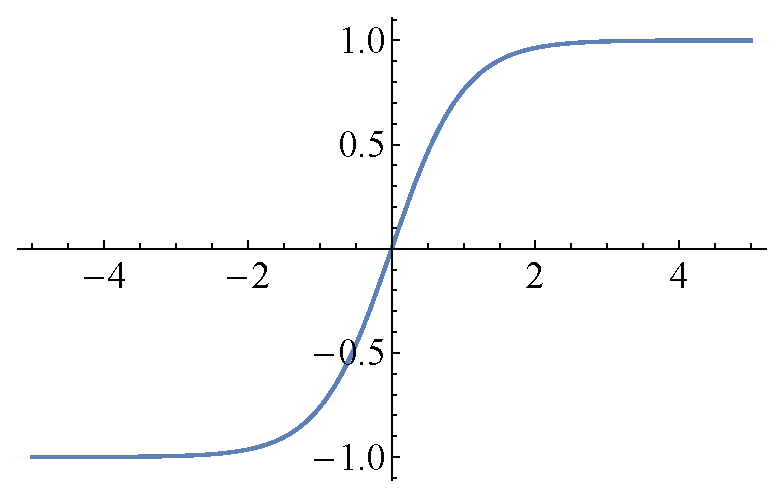
\includegraphics{Figure-5.eps}
		\caption{$f(x)$的一个图像}
	\end{marginfigure}
	令\green{\reff{tanh}}中$\varepsilon\rightarrow 0$,可知$f(x)$可导,且$f'(x)=[1-(f(x))^2]f'(0)$。求解该方程(称为微分方程)可得:$$f(x)=\dfrac{e^{f'(0)x}-e^{-f'(0)x}}{e^{f'(0)x}+e^{-f'(0)x}}=\tanh(f'(0)x)$$		
	至此我们可以发现,函数的基本形态已经大体由②确定了,①中我们只使用了$f(x)$有界这一条件,因此①完全可以放宽为有界性。So what if $f'(0)$ remains undefined?
\end{kaiti}\par\vspace{1em}

\begin{que}
	函数$f(x)$满足①$f(a+b)=f(a)\cdot f(b)$,②$f(4)=16$,$m,n$为互质整数,$n\neq 0$,求$f\left(\dfrac{m}{n}\right)$的值。
\end{que}
\sol 令$a=b=0$得$f(0)=[f(0)]^2\Rightarrow f(0)=0,1$。若$f(0)=0$,再令$b=0$,可得$f(a+0)=f(a)=f(a)f(0)=0\Rightarrow f(x)\equiv 0$,这与②矛盾。以下就$f(0)=1$时情况作讨论。令$b=-a$可得$f(-a)=\dfrac{1}{f(a)}$,再令$a=b=\dfrac{x}{2}$,可得$f(x)=\left[f\left(\dfrac{x}{2}\right)\right]^2\geqslant 0$,再根据条件②可知$f(1)=2$。\par
因此$f\left(\dfrac{m}{n}\right)=\left[f\left(\dfrac{1}{n}\right)\right]^m=\left[f\left(1\right)\right]^{\frac{m}{n}}=\res{2^\frac{m}{n}}$。\par\hfill\tg{抽象函数\ 分析}\easy\par
\begin{kaiti}
	本题中抛却条件②,我们可以知道一个更纯粹的事实:满足$f(a+b)=f(a)\cdot f(b)$的函数$f(x)$至少在有理数域上为指数函数。同\reff{tanh}一样地,我们添加$f(x)$在$x=0$处连续且可导以及全定义域上有界的条件,便可将这一事实拓展到整个实数域(忽略平凡解$f(x)\equiv 0$):注意到随着$\varepsilon\rightarrow 0$,$$|f(x+\varepsilon)-f(x)|=\underbrace{|f(x)|}_{<M}\underbrace{|[f(\varepsilon)-1]|}_{\rightarrow 0}\rightarrow 0$$因此$f(x)$在整个定义域内连续;注意到随着$\varepsilon\rightarrow 0$,
	$$\dfrac{f(x+\varepsilon)-f(x)}{\varepsilon}=f(x)\dfrac{f(\varepsilon)-f(0)}{\varepsilon}\rightarrow f(x)f'(0)<\infty$$因此$f(x)$在整个定义域内可导,且$f'(x)=f(x)f'(0)$,解这一方程可得,$f(x)=e^{f'(0)x}$,这是指数函数。
\end{kaiti}\par

\begin{que}
	已知函数$f(x)$满足:①对任意$x,y\in\mathbb{R}$,有$f(xy)=f(x)f(y)$;②$f(-1)=1$,$f(27)=9$;③$\forall x\in[0,1),f(x)\in[0,1)$。
	\begin{enumerate}
		\item 判断$f(x)$的奇偶性。
		\item 判断$f(x)$在$[0,+\infty)$的单调性。
		\item 若$a\geqslant 0$,且$f(a+1)\leqslant\sqrt[3]{9}$,求$a$的取值范围。
	\end{enumerate}
\end{que}
\sol \begin{enumerate}
	\item 令$y=-1$,得$f(-x)=f(x)f(-1)=f(x)$,$f(x)$为偶函数。
	\item 令$x=y=0$,得$f(0)=0$。$\forall x\in\mathbb{R}^+$,$f(x)=[f(\sqrt{x})]^2\geq 0$。若存在不为零的正实数$x_0$使得$f(x_0)=0$,那末\sidenote{应当注意到,根据题设,$f(x)<\infty$,即$f(x)$定义域为$\mathbb{R}$。}$9=f(27)=f(x_0)f\left(\dfrac{27}{x_0}=0\right)$,矛盾,因此$\forall x>0$,$f(x)>0$。\par
	令$x_1>x_2>0$,$x=x_1$,$y=\dfrac{x_2}{x_1}$,得
	$$f\left(x_1\cdot\dfrac{x_2}{x_1}\right)=\underbrace{f(x_2)}_{>0}=\underbrace{f(x_1)}_{>0}\underbrace{f\left(\dfrac{x_2}{x_1}\right)}_{\in[0,1)}<f(x_1)$$
	因此$f(x)$在$[0,+\infty)$上(严格)单调增,在$(-\infty,0]$上(严格)单调减。
	\item $f((a+1)^2)=[f(a+1)]^3\leqslant 9\ \Leftrightarrow\ (a+1)^3\in[0,27]\ \Leftrightarrow\ \res{a\in[1,2]}$
\end{enumerate}\par\hfill\tg{抽象函数\ 分析}\easy

\begin{que}
	设$A$是定义在$[2,4]$上且满足如下条件的函数$\varphi(x)$的集合:\\
	①\ $\forall x\in[1,2]$,有$\varphi(2x)\in(1,2)$。\\
	②\ 存在常数$L(0<L<1)$,使得对于任意$x_1,x_2\in[1,2]$,都有$|\varphi(2x_1)-\varphi(2x_2)|\leqslant L|x_1-x_2|$。
	\begin{enumerate}
		\item 设$\varphi(2x)=\sqrt[3]{1+x}$,$x\in[2,4]$,证明:$\varphi\in A$。
		\item 设$\varphi\in A$,如果存在$x_0\in(1,2)$,使得$x_0=\varphi(2x_0)$,那么这样的$x_0$是唯一的。
		\item 设$\varphi\in A$,任取$x_1\in(1,2)$,令$x_{n+1}=\varphi(2x_n),n\in\mathbb{N}^+$,证明:给定正整数$k$,那末对于任意的正整数$p$,不等式$$|x_{k+p}-x_{p}|\leqslant \dfrac{L^{k+1}}{1-L}|x_2-x_1|$$成立。
	\end{enumerate}
\end{que}
\sol \begin{enumerate}
	\item \sidenote{本题出题背景涉及到了柯西列、李普希兹条件和柯西中值定理,但最终成题却非常简单。有兴趣可对这些名词稍作了解。应当注意到$\dfrac{f(x_1)-f(x_2)}{x_1-x_2}$为割线斜率。若可导函数割线斜率有界,那末其导函数必有界。}显然$x\in[1,2]$时,$\varphi(2x)=\sqrt[3]{1+x}\in[\sqrt[3]{2},\sqrt[3]{3}]\subset(1,2)$;对于任意$x_1,x_2\in[1,2]$,有
	$$\begin{aligned}
		\left|\sqrt[3]{1+x_1}-\sqrt[3]{1+x_2}\right|&=\dfrac{|x_1-x_2|}{|(1+x_1)^{2/3}+(1+x_2)^{2/3}+(1+x_1)^{1/3}(1+x_2)^{1/3}|}\\
		&\leqslant\dfrac{|x_1-x_2|}{|3\times 2^{2/3}|}=L|x_1-x_2|
	\end{aligned}$$
	其中$L=\dfrac{1}{3\times 2^{2/3}}\in(0,1)$符合要求,因此$\varphi \in A$。
	\item 假设$\exists x_1,x_2\in(1,2)$,$x_1\neq x_2$,$x_1=\varphi(2x_1)$,$x_2=\varphi(2x_2)$,那末
	$|\varphi(2x_1)-\varphi(2x_2)|=|x_1-x_2|$,这与$\varphi(x)\in A$前提下应满足的②矛盾,因此唯一性得以说明。
	\item 注意到这样一个事实:$\forall m\in\mathbb{N}^+$,
	$$|x_{m+1}-x_m|=|\varphi(2x_{m})-\varphi(2x_{m-1})|\leqslant L|x_m-x_{m-1}|\leqslant\cdots\leqslant L^{m-1}|x_2-x_1|$$ 因此,
	$$\begin{aligned}
		|x_{k+p}-x_k|&=|(x_{k+p}-x_{k+p-1})+(x_{k+p-1}-x_{k+p-2})+\cdots+(x_{k+1}-x_k)|\\
		&\leqslant |x_{k+p}-x_{k+p-1}|+|x_{k+p-1}-x_{k+p-2}|+\cdots+|x_{k+1}-x_k|\\
		&\leqslant (L_{k+p-2}+L_{k+p-3}+\cdots+L_{k-1})|x_2-x_1|\\
		&=\dfrac{L_{k-1}(1-L^{p})}{1-L}|x_2-x_1|\\&\leqslant \dfrac{L_{k-1}}{1-L}|x_2-x_1|
	\end{aligned}$$
\end{enumerate}\par\hfill\tg{抽象函数\ 分析}\normal\par

%%%%%%%%%%%%%%%%%%%%%%%%%%%%%%%%%%%%%%%%%%%%%%%%
\section{求取参变量范围的综合题目}
\begin{que}
	已知函数$f(x)=\dfrac{a}{2}x^2+(a+1)x+2\ln(x-1)$,
	\begin{enumerate}
		\item 若曲线$y=f(x)$在点$(2,f(2))$处的切线与直线$2x-y+1=0$平行,求出这条切线的方程。
		\item 讨论函数$f(x)$的单调区间。
		\item 若对于任意$x\in(1,+\infty)$都有$f(x)<-2$,求实数$a$的取值范围。
	\end{enumerate}
\end{que}
\sol 易知$f(x)$定义域$x\in (1,+\infty)$,
	\begin{enumerate}
		\item $f'(x)=ax+a+1+\dfrac{2}{x-1}$$\ \Rightarrow\ $$f'(2)=3a+3=2$,故$a=-\dfrac{1}{3}$,$f(2)=\dfrac{2}{3}$,故切线方程为$$y-\dfrac{2}{3}=2(x-2)\quad\Leftrightarrow\quad \res{3y-6x+10=0}$$
		\item 由于$a=-\dfrac{1}{3}$,故$f(x)=-\dfrac{1}{6}x^2+\dfrac{2}{3}x+2\ln(x-1)$,$f'(x)=-\dfrac{1}{3}x+\dfrac{2}{3}+\dfrac{2}{x-1}$,$f''(x)=-\dfrac{1}{3}-\dfrac{2}{(x-1)^2}<0$,易知%
		$$f'(x)\leqslant 0\ \Leftrightarrow x \in [4,+\infty)\qquad f'(x)\geqslant 0\ \Leftrightarrow x \in (1,4]$$
		故$f(x)$在$(1,4]$上单调增,在$[4,+\infty)$上单调减。
		\item \blue{(方法一)}显然,$a<0$。分离变量得\sidenote{一般都是有两种方法求解此类题。一是将$f(x)$的最大值以$a$表达出来为$g(a)$,再解关于$a$的不等式方程;二是分离变量为$f_1(a) < f_2(x)$后解不等式$f_1(a) < \min f_2(x)$。}
		$$\begin{aligned}\text{原式}\ &\Leftrightarrow\ a(x^2+2x)<-4-2x-4\ln(x-1)\\
			&\Leftrightarrow\ a<-\dfrac{4+2x+4\ln(x-1)}{x^2+2x}=-g(x)\qquad{\purple{\footnotesize{x^2+2x=(x+1)^2-1>3>0}}}\end{aligned}
			$$
		\begin{marginfigure}
			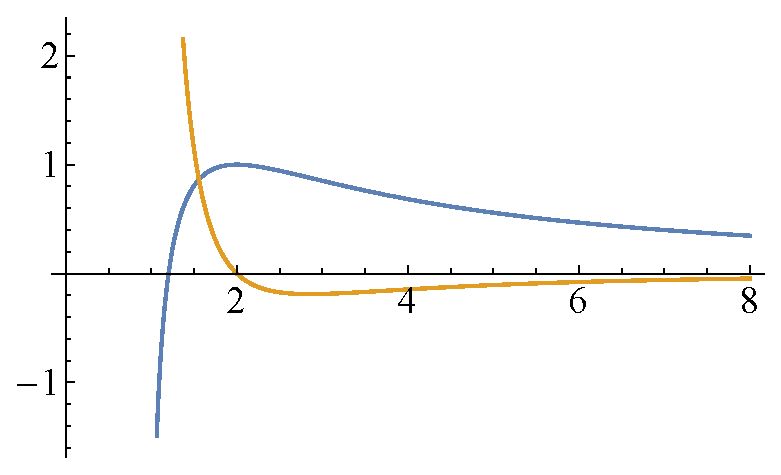
\includegraphics{Figure-1.eps}
			\caption{$g'(x)$的图像}
		\end{marginfigure}
		若我们能够求得$\max g(x)$,则解即为$a < -\max g(x)$。为方便书写,记$\ln0=-\infty$,
		$$g'(x)=-\dfrac{\overbrace{2(x+1)}^{>0}(x^2-4+4(x-1)\ln(x-1))}{\underbrace{x^2(x+2)^2(x-1)}_{>0}}=-\dfrac{2(x+1)(x^2-4+4h(x))}{x^2(x+2)^2(x-1)}$$
		注意到$g'(2)=h(2)=h(1)=0$\ \sidenote{当$x$接近$0$时,$x\ln x$接近$0$。这一点可用不等式$$x-1\geqslant\ln x\geqslant-\dfrac{2}{\sqrt{x}}$$证明。因此我们始终「不妨可设」$0\ln0=0$进行补充定义。为使叙述简便和理解方便,方法一过程中补充定义了边界值,实际考试中应当小心仔细说明。}$g'(2)=h(2)=h(1)=0$。而$h'(x)=\ln(x-1)+1$,故$h(x)$在$\left(1,1+\dfrac{1}{e}\right)$上单调减,在$\left(1+\dfrac{1}{e},+\infty\right)$上单调增,进而$$h(x)<0,x^2-4<0\ \Leftrightarrow\ x\in(1,2)\quad h(x)>0,x^2-4>0\ \Leftrightarrow\ x\in(2,+\infty)$$
		可推知$g(x)$在$(1,2)$上单调增,在$(2,+\infty)$上单调减,$a<-\max g(x)=-g(2)=\res{-1}$。\par\vspace{0.5em}
		\blue{(方法二)}显然,$a<0$。$f'(x)=0\ \Leftrightarrow\ x_1=-1\text{(舍)}\ \ x_2=\dfrac{a-1}{a}>1$,故$f(x)$在$(1,+\infty)$上必然先增后减,
			$$\max f(x)=f\left(\dfrac{a-1}{a}\right)=-1-\dfrac{1}{2a}+\dfrac{3a}{2}+2\ln\left(-\dfrac{1}{a}\right)=g(a)<-2\ \Rightarrow\ a<0$$
			$$g'(a)=\dfrac{3}{2}+\dfrac{1}{2a^2}-\dfrac{2}{a}>0\ \Rightarrow\ g(a)\text{单调增}$$
		注意到$g(-1)=-2$,故所求$a$的取值范围为$\res{a<-1}$。\hfill\tg{参数范围}\easy
	\end{enumerate}

\begin{que}
	设函数$f(x)=2\ln(x-1)-(x-1)^2$,
	\begin{enumerate}
		\item 求函数的单调递增区间。
		\item 若关于函数$x$的方程$f(x)+x^2-3x-a=0$在区间$[2,4]$上有两个相异的实根,求实数$a$的取值范围。
	\end{enumerate}
\end{que}
\sol \begin{enumerate}
	\item $f'(x)=\dfrac{2}{x-1}-2(x-1)$,故结合定义域$x>1$知$f'(x)\geqslant 0\Rightarrow x\in (1,2]$,$f'(x)\leqslant 0\Rightarrow x\in[2,+\infty)$,$f(x)$在$(1,2]$上单调增,在$[2,\infty)$上单调减。
	\item 	
	\begin{marginfigure}
		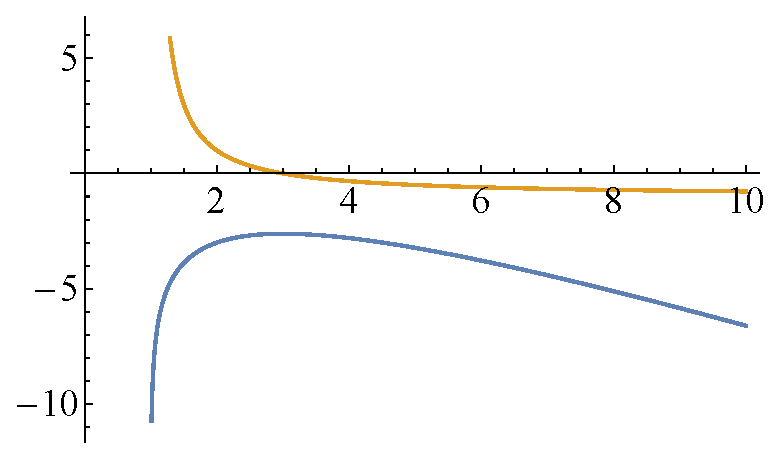
\includegraphics{Figure-2.eps}
		\caption{$g(x)=2\ln(x-1)-x-1$(蓝)及其导函数(橙)的图像}
	\end{marginfigure} 改写原式为$a=f(x)+x^2-3x=2\ln(x-1)-x-1=g(x)$,由$g'(x)=\dfrac{2}{x-1}-1$知
	$$g(x)\text{单调增}\ \Leftrightarrow\ g'(x)\geqslant 0\ \Leftrightarrow x\in(1,3]\quad g(x)\text{单调减}\ \Leftrightarrow\ g'(x)\leqslant 0\ \Leftrightarrow x\in[3,+\infty)$$
	因此$\max g(x)=g(3)=2\ln2-4$。注意到当$x$趋近于$1$或$-\infty$时,$g(x)$均趋近于$-\infty$,我们可大致知道$g(x)$的图像形状,因此易知$a$的取值范围为$\res{a<2\ln2-4}$。\par\vspace{0.5em}\hfill\tg{参数范围\ 最值}\easy
\end{enumerate}
\begin{que}
	已知函数$f(x)=x^3-ax^2-a^2x+1$,$g(x)=1-4x-ax^2$,其中实数$a\neq 0$,
	\begin{enumerate}
		\item 求函数$f(x)$的单调区间。
		\item 当函数$y=f(x)$与$y=g(x)$的图像只有一个公共点且$g(x)$存在最小值时,记$g(x)$的最小值为$h(a)$,求$f(a)$的值域。
		\item 若$f(x)$与$g(x)$在区间$(-a,-a+2)$内均为增函数,求$a$的取值范围。
	\end{enumerate}
\end{que}
\sol \begin{enumerate}
	\item $f'(x)=3x^2-2ax-a^2=(3x+a)(x-a)=0$$\ \Rightarrow\ x_1=-\dfrac{a}{3}$,$x_2=a$,显然$a\neq0$时$x_1\neq x_2$。
	\begin{enumerate}
		\item 当$a>0$时,$x_2>x_1$,$f(x)$在$\left(-\infty,-\dfrac{a}{3}\right]$\textbf{和}$[a,+\infty)$上单调增,在$\left[-\dfrac{a}{3},a\right]$上单调减。
		\item 当$a<0$时,$x_2<x_1$,$f(x)$在$(-\infty,a]$\textbf{和}$\left[-\dfrac{a}{3},+\infty\right)$上单调增,在$\left[a,-\dfrac{a}{3}\right]$上单调减。
	\end{enumerate}
	\item $g(x)$存在最小值意味着$a>0$,由于$f(x)$与$g(x)$的次数不一,因此从两者图像上寻找「只有一个公共点」的情形是困难的,我们须得设差值函数$m(x)=f(x)-g(x)=x^3+(4-a^2)x$,公共点条件即转化为$m(x)$有且仅有一个零点\sidenote{涉及到函数图像相交的问题,均可转化为「交点处为差值函数零点$\Leftrightarrow$交点处函数值相同」的问题,这一过程将减少函数个数,从而简化问题。对于特殊图像,也可从图像特征入手。}。由于$0$为$m(x)$的一个零点,$m(x)$为中心对称的奇函数,故若使$m(x)$零点唯一,$m(x)$必然单调增,即$$m'(0)=[3x^2+(4-a^2)]_{x=0}=4-a^2\geqslant 0\ \Rightarrow\ \res{a\in(0,2]}$$
	\item 记$I=(-a,-a+2)$。$g'(x)=-4-2ax$,使$g(x)$在$I$上单调增有
	$$\left\{\begin{aligned}&g'(-a)=-4+2a^2\geqslant 0\\ &g'(-a+2)=2a^2-4a-4\geqslant 0\end{aligned}\right.\quad\Leftrightarrow\quad a\in(-\infty,-\sqrt{2}]\cup[1+\sqrt{3},+\infty)$$
	在这一范围基础上,注意到$I$的长度为$|I|=2$,而$f'(x)$两根$x_1,x_2$满足$x_1+x_2=\dfrac{2a}{3}$,$x_1x_2=-\dfrac{a^2}{3}$,故$$|x_1-x_2|=\sqrt{(x_1+x_2)^2-4x_1x_2}=\dfrac{4a^2}{3}\geqslant\dfrac{4\times(\sqrt{2})^2}{3}=\dfrac{16}{3}>2=|I|$$
	因此$f(x)$在$I$上不可能有三段增减区间,故只需使
	$$\left\{\begin{aligned}&f'(-a)=4a^2 \geqslant 0\\ &f'(-a+2)=4(a-3)(a-1)\geqslant 0\end{aligned}\right.\quad\Leftrightarrow\quad a\in(-\infty,1]\cup[3,+\infty)$$
	综上,可知$a$的取值范围为$\res{a\in(-\infty,-\sqrt{2}]\cup[3,+\infty)}$。\par\vspace{0.5em}\hfill\tg{取值范围\ 交点}\normal
\end{enumerate}

\begin{que}
	设$a$为实数,记函数$f(x)=a\sqrt{1-x^2}+\sqrt{1+x}+\sqrt{1-x}$的最大值为$g(a)$。
	\begin{enumerate}
		\item 设$t=\sqrt{1+x}+\sqrt{1-x}$,求$t$的取值范围,并把$f(x)$改写为$t$的函数$m(t)$。
		\item 求出$g(a)$。
		\item 求出满足$g(a)=g\left(\dfrac{1}{a}\right)$的所有实数$a$。
	\end{enumerate}
\end{que}
\sol \begin{enumerate}
	\item 显然$x\in [-1,1]$,$t\geqslant 0$,$t^2=2+2\sqrt{1-x^2}\in[2,4]\Rightarrow t\in[\sqrt{2},2]$。同时我们得到$\sqrt{1-x^2}=\dfrac{1}{2}t^2-1$,进而$$f(x)=a\left(\dfrac{1}{2}t^2-1\right)+t=\res{\dfrac{a}{2}t^2+t-a=m(t)}$$
	\item $m(t)$对称轴$t_0=-\dfrac{1}{a}(a\neq 0)$,$t\in[\sqrt{2},2]$。
	\begin{enumerate}
		\item 若$a=0$,则$m(t)$退化为单调增的一次函数\sidenote{一次函数可以视为退化的二次函数,直线和双直线可以视为退化的二次曲线。基于这一点我们应当有这样的先验直觉:$g(a)$必然连续。事实上也的确连续。},最大值$g(0)=m(2)=2$。
		\item 若$a>0$,则$m(t)$为开口向上,对称轴在$y$轴左侧的二次函数,最大值$g(a)=m(2)=a+2$。
		\item 若$a\in\left[-\dfrac{\sqrt{2}}{2},-\dfrac{1}{2}\right]$,则$m(t)$为开口向下,对称轴$t_0\in[\sqrt{2},2]$的二次函数,最大值$g(a)=m(t_0)=-a-\dfrac{1}{2a}$。
		\item 若$a\in\left(-\dfrac{\sqrt{2}}{2},0\right)$,则$m(t)$为开口向下,对称轴$t_0<\sqrt{2}$的二次函数,最大值$g(a)=m(\sqrt{2})=\sqrt{2}$。
		\item 若$a\in\left(-\infty,-\dfrac{1}{2}\right)$,则$m(t)$为开口向下,对称轴$t_0>2$的二次函数,最大值$g(a)=m(2)=2+a$。
	\end{enumerate}
	因此:$g(a)=\left\{\begin{aligned}
		&a+2&a\in\left(-\dfrac{1}{2},+\infty\right)\\
		&-a-\dfrac{1}{2a}&a\in\left[-\dfrac{\sqrt{2}}{2},-\dfrac{1}{2}\right]\\
		&\sqrt{2}&a\in\left(-\infty,-\dfrac{\sqrt{2}}{2}\right)
	\end{aligned}\right.$。\begin{marginfigure}
		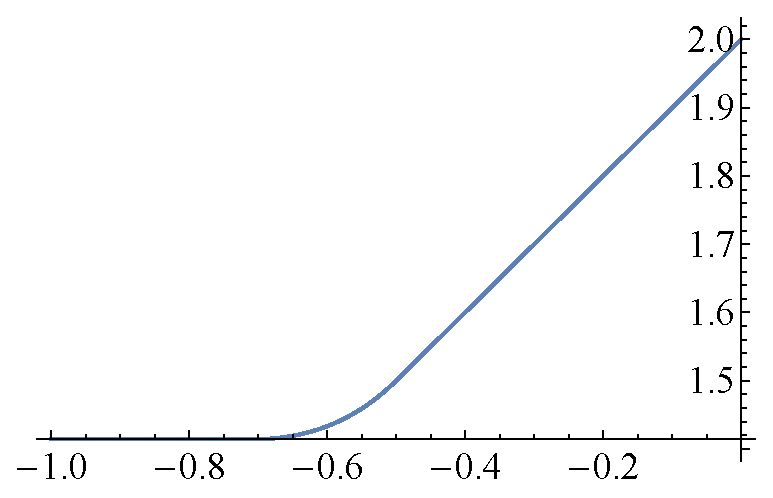
\includegraphics{Figure-4.eps}
		\caption{$g(x)$在$[-1,0]$上的图像。可以看到是连续的。}
	\end{marginfigure}
	\item 由$(a+2)|_{a=-1/2}=\left(-a-\dfrac{1}{2a}\right)|_{a=-1/2}=\dfrac{3}{2}$,$\sqrt{2}=\left(-a-\dfrac{1}{2a}\right)|_{a=-1/\sqrt{2}}=\sqrt{2}$知$g(a)$是连续的。分段求导可知,$g(a)$当$a\geqslant-\dfrac{\sqrt{2}}{2}$时严格单调增,那末
	$$g(a)=g\left(\dfrac{1}{a}\right)\ \Leftrightarrow\ a=\dfrac{1}{a}\text{\ 或\ }a,\dfrac{1}{a}\leqslant-\dfrac{\sqrt{2}}{2}\ \Leftrightarrow\ \res{a\in\left[-\sqrt{2},-\dfrac{\sqrt{2}}{2}\right]\cup\{1\}}$$
\end{enumerate}\par\hfill\tg{取值范围}\easy

\begin{que}
	已知函数$f(x)=\dfrac{1+x}{1-x}e^{-ax}$,
	\begin{enumerate}
		\item 设$a>0$,讨论$y=f(x)$的单调性。
		\item 若对任意$x\in(0,1)$恒有$f(x)>1$,求$a$的取值范围。
	\end{enumerate}
\end{que}
\sol $f'(x)=\dfrac{a\left(x^2+\dfrac{2-a}{a}\right)}{(x-1)^2}e^{-ax}$
\begin{enumerate}
	\item 
	\begin{enumerate}
		\item 若$a\in(0,2]$,则$\dfrac{2-a}{a}\geqslant 0$,$f'(x)\geqslant 0$恒成立,$f(x)$在$(-\infty,1)$\textbf{和}$(1,+\infty)$上单调增。
		\item 若$a>2$,则$f'(x)=0\ \Leftrightarrow\ x_1=-\sqrt{\dfrac{a-2}{a}},\ x_2=\sqrt{\dfrac{a-2}{a}}<1$,因此$f(x)$在$\left(-\infty,-\sqrt{\dfrac{a-2}{a}}\right]$、$\left[\sqrt{\dfrac{a-2}{a}},1\right)$\textbf{和}$(1,+\infty)$上单调增,在$\left[-\sqrt{\dfrac{a-2}{a}},\sqrt{\dfrac{a-2}{a}}\right]$单调减。
	\end{enumerate}
	\item \blue{(方法一)}$(0,1)$上,$f'(x)=\dfrac{2+a\overbrace{(x^2-1)}^{\in(-1,0)}}{(x-1)^2}e^{-ax}$
	\begin{enumerate}
		\item 若$a\leqslant 2$,则$2+a(x^2-1)\geqslant 0\Rightarrow f'(x)$单调增$\Rightarrow f(x)>f(0)=1$,$x\in(0,1)$,这是符合题意的。
		\item 若$a>2$,则$f'(0)<0$,$f(x)$先严格单调减后单调增,而$f(0)=1$,因此必存在$1>x_0>0$\ s.t.\ $f(x_0)<1$,这是不符合题意的,因此$\res{a\leqslant 2}$。
	\end{enumerate}
	\blue{(方法二\ 分离变量法)}易知$x\in(0,1)$则$\dfrac{1+x}{1-x}>0$。$f(x)$取对数知$\forall x\in(0,1)$,$\ln f(x)=\ln(1+x)-\ln(1-x)-ax>\ln 1=0$,
	$$a<\min_{x\in(0,1)}\dfrac{\ln(1+x)}{x}-\dfrac{\ln(1-x)}{x}=\min_{x\in(0,1)} g(x)$$
	$g'(x)=\dfrac{1}{x^2}\left[\dfrac{2x}{1-x^2}+\ln\left(\dfrac{1-x}{1+x}\right)\right]=\dfrac{1}{x^2}h(x)$,注意到$h'(x)=\dfrac{4x^2}{(x^2-1)^2}>0$,$h(0)=0$,故在$(0,1)$上$g'(x)>0$,$g(x)$单调增。现在我们须找出$x$趋近于$0$时,$g(x)$趋近的值。事实上,可利用以下不等式\sidenote{这里的不等式均源于多项式级数展开的截取,证明大同小异,非常简单,故不再证明。下诸题同。}:
	$$\begin{aligned}&\quad x-\dfrac{x^2}{2}\leqslant\ln(1+x)\leqslant x\\
		&\Rightarrow\ \left(x-\dfrac{x^2}{2}\right)-(-x)\leqslant\ln(1+x)-\ln(1-x)\leqslant x-\left(-x-\dfrac{x^2}{2}\right)\\
		&\Leftrightarrow 2x-\dfrac{x^2}{2}\leqslant\ln\left(\dfrac{1+x}{1-x}\right)\leqslant 2x+\dfrac{x^2}{2}\qquad\purple{\text{\footnotesize 这是一个非常常用的不等式}}\\
		&\Leftrightarrow 2-\dfrac{x}{2}\leqslant g(x)\leqslant 2+\dfrac{x}{2}\end{aligned}$$
	因此\sidenote{「趋于」这一词引入于数学教材定积分一章,是否在考试中可以使用视要求而定。不能使用的情况下可以如下叙述:\begin{enumerate}
		\item $g(x)$是连续的,且单调增至无穷。对于任意大于$2$的值,譬如$2+\epsilon$,$\epsilon>0$,均可取适当的$x>0$,使得$g(x)\leqslant 2+\dfrac{x^2}{2} < 2+\epsilon$,这样由$g(x)$单调增知$g(x)$必可取到$2+\epsilon$。
		\item 假设$g(x)$可取到任意小于$2$的值,譬如$g(x_0)=2-\epsilon$,$\epsilon>0$,均可取适当的$x_0>x_1>0$,使得$g(x_1)\geqslant 2-\dfrac{x^2}{2} > 2-\epsilon$,这与$g(x)$单调增矛盾。
		\item 因此$g(x)$必然严格大于$2$。
	\end{enumerate}}当$x$趋于$0$时,$g(x)$趋于$2$,而这一最小值是取不到的。因此$\res{a\leqslant 2}$。
\end{enumerate}\par\hfill\gk\tg{取值范围\ 极限}\easy

%%%%%%%%%%%%%%%%%%%%%%%%%%%%%%%%%%%%%%%%%%%%%%%%
\section{引出不等式证明的综合题目}
关于此类题目一些常用不等式的统一证明:
\begin{enumerate}
	\item \labeltext[[IEQ\ 1]]{$\mathbf{e^x\geqslant 1+x}$}{ieq1} \par
	该式截取自$e^x$的麦克劳林展开式$$e^x=1+x+\dfrac{x^2}{2!}+\dfrac{x^3}{3!}+\cdots+\dfrac{x^n}{n!}+\cdots$$前两项,截取更多项时证明相仿,只需多求几次导数,不赘述。\par
	令$g(x)=e^x-(1+x)$,则$g'(x)=e^x-1$,$g''(x)=e^x>0$,因此$g'(x)$单调增,又$g'(0)=0$,因此$g(x)$在$(-\infty,0)$上单调递减,在$(0,+\infty)$上单调递增,$\forall x\in\mathbb{R}$,$$g(x)\geqslant g(0)=0\ \Leftrightarrow\ e^x\geqslant 1+x$$
	当仅当$x=0$时取等。
	 \item \labeltext[[IEQ\ 2]]{$\mathbf{\ln(1+x)\leqslant x(x>-1),\ln(1+x)\geqslant x-\dfrac{x^2}{2}}(x\geqslant 0)$}{ieq2} \par
	该式截取自$\ln(1+x)$的麦克劳林展开式$$\ln(1+x)=x-\dfrac{x^2}{2}+\dfrac{x^3}{3}-\cdots+(-1)^{n+1}\dfrac{x^n}{n}+\cdots$$前两项,截取更多项时证明相仿,只需多求几次导数,不赘述,这里我们证第二式。\par
	令$g(x)=\ln(1+x)-x+\dfrac{x^2}{2!}$,则$g'(x)=\dfrac{1}{1+x}-1+x$,$g''(x)=-\dfrac{1}{(1+x)^2}+1\geqslant 0$,$g'(0)=0$,因此$g(x)$在$[0,+\infty)$上单调增,$\forall x\geqslant 0$,$$g(x)\geqslant 0 \ \Rightarrow\ \ln(1+x)\geqslant x-\dfrac{x^2}{2}$$
	当仅当$x=0$时取等。
	%\item \labeltext[[IEQ\ 3]]{$\mathbf{\ }$}{ieq2} \par
\end{enumerate}
\begin{que}
	已知函数$f(x)=\dfrac{a(1-x)}{x}\ln(1-x),a\in\mathbb{R}$,$e$为自然常数。
	\begin{enumerate}
		\item 求$f(x)$在区间$\left[1-e^2,1-e\right]$上的最值。
		\item 比较$\left(1+\dfrac{1}{2!}\right)\left(1+\dfrac{1}{3!}\right)\cdots\left(1+\dfrac{1}{n!}\right)$与$e$的大小。
	\end{enumerate}
\end{que}
\sol \begin{enumerate}
	\item 导数$f'(x)=-\dfrac{a(x+\ln(1-x))}{x^2}$。由\ref{ieq2},$\ln(1-x)\leqslant -x$,因此
	\begin{enumerate}
		\item 若$a=0$,则$f(x)\equiv 0$,所求最值$\res{\max f(x)=0}$。
		\item 若$a>0$,则$x+\ln(1-x)\leqslant 0$,$f'(x)\geqslant 0$,$f(x)$单调增,所求最值
		$$\max_{[1-e^2,1-e]} f(x)=f(1-e)=\res{\dfrac{ae}{1-e}}\quad \min_{[1-e^2,1-e]}f(x)=f(1-e^2)=\res{\dfrac{2ae^2}{1-e^2}}$$
		 \item 若$a<0$,则$f'(x)\leqslant 0$,$f(x)$单调减,所求最值
		$$\min_{[1-e^2,1-e]} f(x)=f(1-e)=\res{\dfrac{ae}{1-e}}\quad \max_{[1-e^2,1-e]}f(x)=f(1-e^2)=\res{\dfrac{2ae^2}{1-e^2}}$$
	\end{enumerate}
\end{enumerate}

什么\textbf{什么}\textsf{什么}\textit{什么}\textrm{什么}\textsc{什么}\textsl{什么}\texttt{什么}\tg{参数范围}\easy
Many modern printed textbooks have adopted a layout with prominent 
margins where small figures, tables, remarks and just about everything 
else can be displayed. Arguably, this layout helps to organise the 
	discussion by separating the main text from the ancillary material, 
	which at the same time is very close to the point in the text where 
	it is referenced.

This document does not aim to be an apology of wide margins, for there 
are many better suited authors for this task; the purpose of all these 
words is just to fill the space so that the reader can see how a book 
written with the kaobook class looks like. Meanwhile, I shall also try 
to illustrate the features of the class.

The main ideas behind kaobook come from this 
\href{https://3d.bk.tudelft.nl/ken/en/2016/04/17/a-1.5-column-layout-in-latex.html}{blog 
	post}, and actually the name of the class is dedicated to the author 
of the post, Ken Arroyo Ohori, which has kindly allowed me to create a 
class based on his thesis. Therefore, if you want to know more reasons 
to prefer a 1.5-column layout for your books, be sure to read his blog 
post.

Another source of inspiration, as you may have noticed, is the 
\href{https://github.com/Tufte-LaTeX/tufte-latex}{Tufte-Latex Class}. 
The fact that the design is similar is due to the fact that it is very 
difficult to improve something which is already so good. However, I like 
to think that this class is more flexible than Tufte-Latex. For 
instance, I have tried to use only standard packages and to implement as 
little as possible from scratch;\sidenote{This also means that 
understanding and contributing to the class development is made easier. 
Indeed, many things still need to be improved, so if you are interested, 
check out the repository on github!} therefore, it should be pretty easy 
to customise anything, provided that you read the documentation of the 
package that provides that feature.

In this book I shall illustrate the main features of the class and 
provide information about how to use and change things. Let us get 
started.

\section{What This Class Does}
\labsec{does}

The \Class{kaobook} class focuses more about the document structure than 
about the style. Indeed, it is a well-known \LaTeX\xspace principle that 
structure and style should be separated as much as possible (see also 
\vrefsec{doesnot}). This means that this class will only provide 
commands, environments and in general, the opportunity to do things, 
which the user may or may not use. Actually, some stylistic matters are 
embedded in the class, but the user is able to customise them with ease.

The main features are the following:

\begin{description}
	\item[Page Layout] The text width is reduced to improve readability 
	and make space for the margins, where any sort of elements can be 
	displayed.
	\item[Chapter Headings] As opposed to Tufte-Latex, we provide a 
	variety of chapter headings among which to choose; examples will be 
	seen in later chapters.
	\item[Page Headers] They span the whole page, margins included, and, 
	in twoside mode, display alternatively the chapter and the section 
	name.\sidenote[][-2mm]{This is another departure from Tufte's 
	design.}
	\item[Matters] The commands \Command{frontmatter}, 
	\Command{mainmatter} and \Command{backmatter} have been redefined in 
	order to have automatically wide margins in the main matter, and 
	narrow margins in the front and back matters. However, the page 
	style can be changed at any moment, even in the middle of the 
	document.
	\item[Margin text] We provide commands \Command{sidenote} and 
	\Command{marginnote} to put text in the 
	margins.\sidenote[][-2mm]{Sidenotes (like this!) are numbered while 
	marginnotes are not}
	\item[Margin figs/tabs] A couple of useful environments is 
	\Environment{marginfigure} and \Environment{margintable}, which, not 
	surprisingly, allow you to put figures and tables in the margins 
	(\cfr \reffig{marginmonalisa}).
	\item[Margin toc] Finally, since we have wide margins, why don't add 
	a little table of contents in them? See \Command{margintoc} for 
	that.
	\item[Hyperref] \Package{hyperref} is loaded and by default we try 
	to add bookmarks in a sensible way; in particular, the bookmarks 
	levels are automatically reset at \Command{appendix} and 
	\Command{backmatter}. Moreover, we also provide a small package to 
	ease the hyperreferencing of other parts of the text.
	\item[Bibliography] We want the reader to be able to know what has 
	been cited without having to go to the end of the document every 
	time, so citations go in the margins as well as at the end, as in 
	Tufte-Latex. Unlike that class, however, you are free to customise 
	the citations as you wish.
\end{description}

\begin{marginfigure}[-5.5cm]
	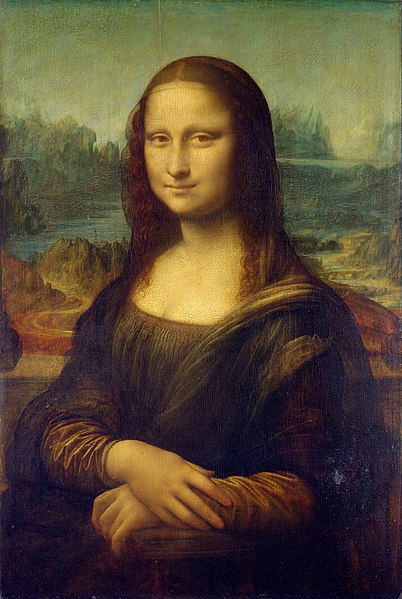
\includegraphics{monalisa}
	\caption[The Mona Lisa]{The Mona Lisa.\\ 
	\url{https://commons.wikimedia.org/wiki/File:Mona_Lisa,_by_Leonardo_da_Vinci,_from_C2RMF_retouched.jpg}}
	\labfig{marginmonalisa}
\end{marginfigure}

The order of the title pages, table of contents and preface can be 
easily changed, as in any \LaTeX\ document. In addition, the class is 
based on \KOMAScript's \Class{scrbook}, therefore it inherits all the 
goodies of that.

\section{What This Class Does Not Do}
\labsec{doesnot}

As anticipated, further customisation of the book is left to the user. 
Indeed, every book may have sidenotes, margin figures and so on, but 
each book will have its own fonts, toc style, special environments and 
so on. For this reason, in addition to the class, we provide only 
sensible defaults, but if these features are not needed, they can be 
left out. These special packages are located in the \Path{style} 
directory, which is organised as follows:

\begin{description}
	\item[kao.sty] This package contains the most important definitions 
	of macros and specifications of page layout. It is the heart of the 
	\Class{kaobook}.
	\item[kaobiblio.sty] Contains commands to add citations and 
	customise the bibliography.
	\item[packages.sty] Loads additional packages to decorate the 
	writing with special contents (for instance, the \Package{listing} 
	package is loaded here as it is not required in every book). There 
	are also defined some useful commands to print the same words always 
	in the same way, \eg latin words in italics or \Package{packages} in 
	verbatim.
	\item[kaorefs.sty] Some useful commands to manage labeling and 
	referencing, again to ensure that the same elements are referenced 
	always in a consistent way.
	\item[environments.sty] Provides special environments, like boxes. 
	Both simple and complex environments are available; by complex we 
	mean that they are endowed with a counter, floating and can be put 
	in a special table of contents.\sidenote[][-2mm]{See 
	\vrefch{mathematics} for some examples.}
	\item[theorems.sty] The style of mathematical environments. 
	Actually, there are two such packages: one is for plain theorems,
	\ie the theorems are printed in plain text; the other uses 
	\Package{mdframed} to draw a box around theorems. You can plug the 
	most appropriate style into its document.
\end{description}

\marginnote[2mm]{The audacious users might feel tempted to edit some of 
these packages. I'd be immensely happy if they sent me examples of what 
they have been able to do!}

In the rest of the book, I shall assume that the reader is not a novice 
in the use of \LaTeX, and refer to the documentation of the packages 
used in this class for things that are already explained there. 
Moreover, I assume that the reader is willing to make minor edits to the 
provided packages for styles, environments and commands, if he or she 
does not like the default settings.

\section{How to Use This Class}

Either if you are using the template from 
\href{http://latextemplates.org/template/kaobook}{latextemplates}, or if 
you cloned the GitHub 
\href{https://www.github.com/fmarotta/kaobook}{repository}, there are 
infinite ways to use the \Class{kaobook} class in practice, but we will 
discuss only two of them. The first is to find the \Path{main.tex} file 
which I used to write this book, and edit it; this will probably involve 
a lot of text-deleting, copying-and-pasting, and rewriting. The second 
way is to start almost from scratch and use the \Path{skeleton.tex} 
file, which is a cleaned-up version of the \Path{main.tex}; even if you 
choose the second way, you may find it useful to draw inspiration from 
the \Path{main.tex} file.

To compile the document, assuming that its name is \Path{main.tex}, you 
will have to run the following sequence of commands:

\begin{lstlisting}[style=kaolstplain,linewidth=1.5\textwidth]
pdflatex main # Compile template
makeindex main.nlo -s nomencl.ist -o main.nls # Compile nomenclature
makeindex main # Compile index
biber main # Compile bibliography
makeglossaries main # Compile glossary
pdflatex main # Compile template again
pdflatex main # Compile template again
\end{lstlisting}

You may need to compile the template some more times in order for some 
errors to disappear. For any support requests, please ask a question on 
\url{tex.stackexchange.org} with the tag \enquote{kaobook}, open an 
issue on GitHub, or contact the author via e-mail.
